% Options for packages loaded elsewhere
\PassOptionsToPackage{unicode}{hyperref}
\PassOptionsToPackage{hyphens}{url}
%
\documentclass[
]{book}
\usepackage{amsmath,amssymb}
\usepackage{lmodern}
\usepackage{iftex}
\ifPDFTeX
  \usepackage[T1]{fontenc}
  \usepackage[utf8]{inputenc}
  \usepackage{textcomp} % provide euro and other symbols
\else % if luatex or xetex
  \usepackage{unicode-math}
  \defaultfontfeatures{Scale=MatchLowercase}
  \defaultfontfeatures[\rmfamily]{Ligatures=TeX,Scale=1}
\fi
% Use upquote if available, for straight quotes in verbatim environments
\IfFileExists{upquote.sty}{\usepackage{upquote}}{}
\IfFileExists{microtype.sty}{% use microtype if available
  \usepackage[]{microtype}
  \UseMicrotypeSet[protrusion]{basicmath} % disable protrusion for tt fonts
}{}
\makeatletter
\@ifundefined{KOMAClassName}{% if non-KOMA class
  \IfFileExists{parskip.sty}{%
    \usepackage{parskip}
  }{% else
    \setlength{\parindent}{0pt}
    \setlength{\parskip}{6pt plus 2pt minus 1pt}}
}{% if KOMA class
  \KOMAoptions{parskip=half}}
\makeatother
\usepackage{xcolor}
\usepackage{color}
\usepackage{fancyvrb}
\newcommand{\VerbBar}{|}
\newcommand{\VERB}{\Verb[commandchars=\\\{\}]}
\DefineVerbatimEnvironment{Highlighting}{Verbatim}{commandchars=\\\{\}}
% Add ',fontsize=\small' for more characters per line
\usepackage{framed}
\definecolor{shadecolor}{RGB}{248,248,248}
\newenvironment{Shaded}{\begin{snugshade}}{\end{snugshade}}
\newcommand{\AlertTok}[1]{\textcolor[rgb]{0.94,0.16,0.16}{#1}}
\newcommand{\AnnotationTok}[1]{\textcolor[rgb]{0.56,0.35,0.01}{\textbf{\textit{#1}}}}
\newcommand{\AttributeTok}[1]{\textcolor[rgb]{0.77,0.63,0.00}{#1}}
\newcommand{\BaseNTok}[1]{\textcolor[rgb]{0.00,0.00,0.81}{#1}}
\newcommand{\BuiltInTok}[1]{#1}
\newcommand{\CharTok}[1]{\textcolor[rgb]{0.31,0.60,0.02}{#1}}
\newcommand{\CommentTok}[1]{\textcolor[rgb]{0.56,0.35,0.01}{\textit{#1}}}
\newcommand{\CommentVarTok}[1]{\textcolor[rgb]{0.56,0.35,0.01}{\textbf{\textit{#1}}}}
\newcommand{\ConstantTok}[1]{\textcolor[rgb]{0.00,0.00,0.00}{#1}}
\newcommand{\ControlFlowTok}[1]{\textcolor[rgb]{0.13,0.29,0.53}{\textbf{#1}}}
\newcommand{\DataTypeTok}[1]{\textcolor[rgb]{0.13,0.29,0.53}{#1}}
\newcommand{\DecValTok}[1]{\textcolor[rgb]{0.00,0.00,0.81}{#1}}
\newcommand{\DocumentationTok}[1]{\textcolor[rgb]{0.56,0.35,0.01}{\textbf{\textit{#1}}}}
\newcommand{\ErrorTok}[1]{\textcolor[rgb]{0.64,0.00,0.00}{\textbf{#1}}}
\newcommand{\ExtensionTok}[1]{#1}
\newcommand{\FloatTok}[1]{\textcolor[rgb]{0.00,0.00,0.81}{#1}}
\newcommand{\FunctionTok}[1]{\textcolor[rgb]{0.00,0.00,0.00}{#1}}
\newcommand{\ImportTok}[1]{#1}
\newcommand{\InformationTok}[1]{\textcolor[rgb]{0.56,0.35,0.01}{\textbf{\textit{#1}}}}
\newcommand{\KeywordTok}[1]{\textcolor[rgb]{0.13,0.29,0.53}{\textbf{#1}}}
\newcommand{\NormalTok}[1]{#1}
\newcommand{\OperatorTok}[1]{\textcolor[rgb]{0.81,0.36,0.00}{\textbf{#1}}}
\newcommand{\OtherTok}[1]{\textcolor[rgb]{0.56,0.35,0.01}{#1}}
\newcommand{\PreprocessorTok}[1]{\textcolor[rgb]{0.56,0.35,0.01}{\textit{#1}}}
\newcommand{\RegionMarkerTok}[1]{#1}
\newcommand{\SpecialCharTok}[1]{\textcolor[rgb]{0.00,0.00,0.00}{#1}}
\newcommand{\SpecialStringTok}[1]{\textcolor[rgb]{0.31,0.60,0.02}{#1}}
\newcommand{\StringTok}[1]{\textcolor[rgb]{0.31,0.60,0.02}{#1}}
\newcommand{\VariableTok}[1]{\textcolor[rgb]{0.00,0.00,0.00}{#1}}
\newcommand{\VerbatimStringTok}[1]{\textcolor[rgb]{0.31,0.60,0.02}{#1}}
\newcommand{\WarningTok}[1]{\textcolor[rgb]{0.56,0.35,0.01}{\textbf{\textit{#1}}}}
\usepackage{longtable,booktabs,array}
\usepackage{calc} % for calculating minipage widths
% Correct order of tables after \paragraph or \subparagraph
\usepackage{etoolbox}
\makeatletter
\patchcmd\longtable{\par}{\if@noskipsec\mbox{}\fi\par}{}{}
\makeatother
% Allow footnotes in longtable head/foot
\IfFileExists{footnotehyper.sty}{\usepackage{footnotehyper}}{\usepackage{footnote}}
\makesavenoteenv{longtable}
\usepackage{graphicx}
\makeatletter
\def\maxwidth{\ifdim\Gin@nat@width>\linewidth\linewidth\else\Gin@nat@width\fi}
\def\maxheight{\ifdim\Gin@nat@height>\textheight\textheight\else\Gin@nat@height\fi}
\makeatother
% Scale images if necessary, so that they will not overflow the page
% margins by default, and it is still possible to overwrite the defaults
% using explicit options in \includegraphics[width, height, ...]{}
\setkeys{Gin}{width=\maxwidth,height=\maxheight,keepaspectratio}
% Set default figure placement to htbp
\makeatletter
\def\fps@figure{htbp}
\makeatother
\setlength{\emergencystretch}{3em} % prevent overfull lines
\providecommand{\tightlist}{%
  \setlength{\itemsep}{0pt}\setlength{\parskip}{0pt}}
\setcounter{secnumdepth}{5}
\usepackage{booktabs}
\ifLuaTeX
  \usepackage{selnolig}  % disable illegal ligatures
\fi
\usepackage[]{natbib}
\bibliographystyle{apalike}
\IfFileExists{bookmark.sty}{\usepackage{bookmark}}{\usepackage{hyperref}}
\IfFileExists{xurl.sty}{\usepackage{xurl}}{} % add URL line breaks if available
\urlstyle{same} % disable monospaced font for URLs
\hypersetup{
  pdftitle={初級統計学},
  pdfauthor={TI},
  hidelinks,
  pdfcreator={LaTeX via pandoc}}

\title{初級統計学}
\author{TI}
\date{2023-03-08}

\usepackage{amsthm}
\newtheorem{theorem}{Theorem}[chapter]
\newtheorem{lemma}{Lemma}[chapter]
\newtheorem{corollary}{Corollary}[chapter]
\newtheorem{proposition}{Proposition}[chapter]
\newtheorem{conjecture}{Conjecture}[chapter]
\theoremstyle{definition}
\newtheorem{definition}{Definition}[chapter]
\theoremstyle{definition}
\newtheorem{example}{Example}[chapter]
\theoremstyle{definition}
\newtheorem{exercise}{Exercise}[chapter]
\theoremstyle{definition}
\newtheorem{hypothesis}{Hypothesis}[chapter]
\theoremstyle{remark}
\newtheorem*{remark}{Remark}
\newtheorem*{solution}{Solution}
\begin{document}
\maketitle

{
\setcounter{tocdepth}{1}
\tableofcontents
}
\hypertarget{ux7de8ux96c6ux7528}{%
\chapter*{編集用}\label{ux7de8ux96c6ux7528}}
\addcontentsline{toc}{chapter}{編集用}

\url{https://bookdown.org/yihui/rmarkdown-cookbook/}

Qiita マークダウン記法 一覧表・チートシート
\url{https://qiita.com/kamorits/items/6f342da395ad57468ae3}

This is a \emph{sample} book written in \textbf{Markdown}. You can use anything that Pandoc's Markdown supports; for example, a math equation \(a^2 + b^2 = c^2\).

\hypertarget{usage}{%
\section{Usage}\label{usage}}

Each \textbf{bookdown} chapter is an .Rmd file, and each .Rmd file can contain one (and only one) chapter. A chapter \emph{must} start with a first-level heading: \texttt{\#\ A\ good\ chapter}, and can contain one (and only one) first-level heading.

Use second-level and higher headings within chapters like: \texttt{\#\#\ A\ short\ section} or \texttt{\#\#\#\ An\ even\ shorter\ section}.

The \texttt{index.Rmd} file is required, and is also your first book chapter. It will be the homepage when you render the book.

\hypertarget{render-book}{%
\section{Render book}\label{render-book}}

You can render the HTML version of this example book without changing anything:

\begin{enumerate}
\def\labelenumi{\arabic{enumi}.}
\item
  Find the \textbf{Build} pane in the RStudio IDE, and
\item
  Click on \textbf{Build Book}, then select your output format, or select ``All formats'' if you'd like to use multiple formats from the same book source files.
\end{enumerate}

Or build the book from the R console:

\begin{Shaded}
\begin{Highlighting}[]
\NormalTok{bookdown}\SpecialCharTok{::}\FunctionTok{render\_book}\NormalTok{()}
\end{Highlighting}
\end{Shaded}

To render this example to PDF as a \texttt{bookdown::pdf\_book}, you'll need to install XeLaTeX. You are recommended to install TinyTeX (which includes XeLaTeX): \url{https://yihui.org/tinytex/}.

\hypertarget{preview-book}{%
\section{Preview book}\label{preview-book}}

As you work, you may start a local server to live preview this HTML book. This preview will update as you edit the book when you save individual .Rmd files. You can start the server in a work session by using the RStudio add-in ``Preview book'', or from the R console:

\begin{Shaded}
\begin{Highlighting}[]
\NormalTok{bookdown}\SpecialCharTok{::}\FunctionTok{serve\_book}\NormalTok{()}
\end{Highlighting}
\end{Shaded}

\hypertarget{part-ux7b2cuxff11ux90e8}{%
\chapter{(PART*) 第1部}\label{part-ux7b2cuxff11ux90e8}}

\hypertarget{ux7d71ux8a08ux3068ux4ebaux9593ux751fux6d3b}{%
\chapter{統計と人間生活}\label{ux7d71ux8a08ux3068ux4ebaux9593ux751fux6d3b}}

日常生活では\textbf{統計的な考え方}がさまざまな場面で利用されている

\begin{quote}
例1:統計がないとスポーツ観戦がつまらなくなる
野球では,過去の対戦成績(○勝△敗),打撃成績(○割○分○厘),投手成績(防御率)のような\textbf{統計}が利用される

\[
\text{打率}=\frac{\text{安打}}{\text{打数}} \qquad\qquad
\text{防御率}=\frac{\text{自責点}}{\text{投球回}} \times 9
\]
\end{quote}

これらの\textbf{統計}が存在しなければ:

\begin{itemize}
\tightlist
\item
  登場した打者にどれくらいの安打が期待できるのかわからない
\item
  投手にどれくらいの健闘が期待できるのかわからない
\end{itemize}

\begin{quote}
例2:統計がないと今日の天気を比べられない
天気予報で気象予報士が「きょうは4月中旬にしては異常に暖かかった」あるいは「きょうは6月上旬の陽気であった」と表現することがある。
\end{quote}

\begin{itemize}
\tightlist
\item
  「異常」な状態を定義するには,「平常」な状態の定義が必要
\item
  ではどのように「平常」な状態を定義できるだろうか?
\item
  「平常」な気温は,過去何十年にもわたって観測した4月中旬の気温を平均してもとめた\underline{平均気温}という統計数字
\item
  「異常」な暖かさとは「平常」な気温の値があってはじめて判断できる
\item
  疑問:平均気温よりもどれくらい離れていると「異常」と言えるだろうか?
\end{itemize}

\begin{quote}
例3:統計がなければ「当選確実」かどうかはすぐにわからない
選挙速報で,数パーセントしか開票していないのに「当選確実」と報道できるのはなぜか?
\end{quote}

\begin{itemize}
\tightlist
\item
  選挙前の支持者,投票意向などの統計的調査などから得た情報をもとに``推定'\,'
\item
  \textbf{一部分の開票結果}から\textbf{全体の傾向}を推しはかる``統計的推論'\,'とよばれる分析の応用例
\end{itemize}

\begin{quote}
例4:企業経営に統計は不可欠
多くの製造業者は,注文を受けてから製品を製造する\textbf{受注生産}ではなく,どれくらい売れそうかという見込みをたてて製品を製造する\textbf{見込生産}を行っている
\end{quote}

\begin{itemize}
\tightlist
\item
  生産量が多すぎれば\textbf{在庫}を抱えてしまうし,少なすぎたりすると社会的に混乱を生じさせてしまう

  \begin{itemize}
  \tightlist
  \item
    例:食品メーカーのある炭酸飲料が「予想を上回る注文があったため販売2日目で当面出荷停止」
  \item
    サントリーのオランジーナ 2015/4/2
  \end{itemize}
\item
  人口総数,男女別構成・年齢別構成等の統計をもとに需要予測を行い,生産量の計画をたてる
\item
  消費者の消費習慣や購買習慣を,企業みずから,あるいは専門の調査機関に依頼して\textbf{市場調査}する
\end{itemize}

\begin{quote}
例5:経済政策の決定にも統計は不可欠
政府は所得税を減税することで消費を増加させ,公共投資を増やすことによって景気を刺激しようとする。政策を決定する際には,各種の経済統計(家計調査,設備投資計画調査など)が示す経済状態に細心の注意を払うと同時に,各種税率,公共投資額,金利,マネーストック等の経済政策にかかわる変数と経済の状態を示す各種変数との関係が利用されている
\end{quote}

\begin{itemize}
\tightlist
\item
  GDP,物価指数,金利,株価,失業率,為替レートなどのマクロ経済データを使って作成した計量経済学的モデルは,政府の経済政策の決定に不可欠なツールのひとつ
\end{itemize}

\begin{quote}
内閣府の経済社会総合研究所の分析(2015)

\begin{itemize}
\tightlist
\item
  消費税率1\%引上げで1年後の実質GDPは0.24\%減少
\item
  短期金利1\%引上げで1年後の実質GDPは0.32\%減少
\item
  内閣府経済社会総合研究所「短期日本経済マクロ計量モデル(2015年版)の構造と乗数分析」
  \%(\url{http://www.esri.go.jp/jp/archive/e/_dis/e/_dis314/e/_dis314.pdf})
\end{itemize}
\end{quote}

\begin{quote}
例6:アパート・マンションを選ぶときにも統計が使える
この部屋の家賃は平均よりも高いのか、それとも安いのか?
\end{quote}

\begin{figure}
\centering
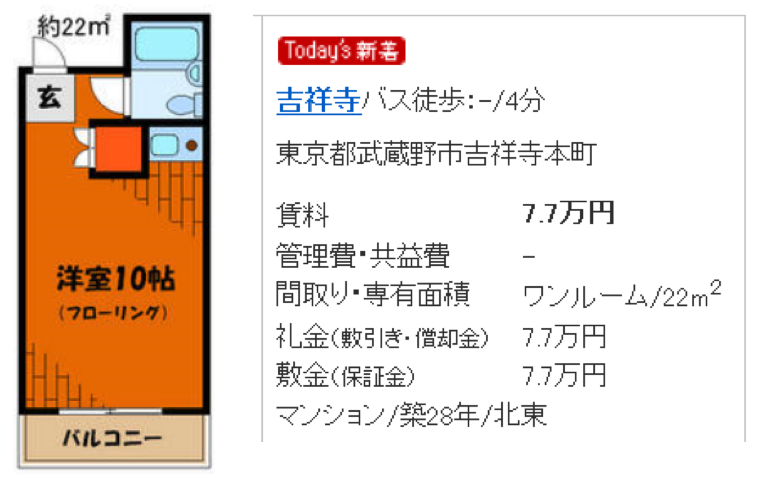
\includegraphics[width=0.5\textwidth,height=\textheight]{images/lec01/fig_kichi_1room_example.png}
\caption{image of histogram}
\end{figure}

\hypertarget{ux7d71ux8a08ux3068ux306f}{%
\section{統計とは}\label{ux7d71ux8a08ux3068ux306f}}

\begin{quote}
統計とは
統計とは,ある特定の集団について,それを構成するものの特定の性質に注目して観察し,その集団全体の特徴を数量的に表現しようとするもの
\end{quote}

\begin{itemize}
\tightlist
\item
  \textbf{記述統計}:複数の者,あるいは複数の時点で示した数字を集約整理し,その集団全体の\textbf{特徴を示そうとする}もの
\item
  \textbf{推測統計}:一部から全体の\textbf{特徴を推測・予測する}こと
\end{itemize}

\begin{quote}
質問
先述の例を分類してみましょう

\begin{longtable}[]{@{}ccc@{}}
\toprule()
& テーマ & 種類 \\
\midrule()
\endhead
例1 & スポーツ観戦 & データの要約(平均的傾向),記述 \\
例2 & 異常な天気 & データの要約(ちらばり具合) \\
例3 & 選挙速報 & 予測,推定 \\
例4 & 見込み生産 & 予測,推定 \\
例5 & 経済政策 & 記述,推定 \\
\bottomrule()
\end{longtable}
\end{quote}

\hypertarget{ux30c7ux30fcux30bfux306eux5c3aux5ea6ux306aux3069}{%
\chapter{データの尺度など}\label{ux30c7ux30fcux30bfux306eux5c3aux5ea6ux306aux3069}}

\hypertarget{ux30c7ux30fcux30bfux306eux5c3aux5ea6}{%
\section{データの尺度}\label{ux30c7ux30fcux30bfux306eux5c3aux5ea6}}

\begin{itemize}
\tightlist
\item
  データを作りあげている値にはさまざまな種類がある
\end{itemize}

\begin{quote}
例:ある大学の学生の成績・個人情報にかかわるデータ
\end{quote}

\begin{longtable}[]{@{}lllllll@{}}
\toprule()
学生ID & 学年 & 英語 & ミクロ & \(\cdots\) & GPA & 通学時間(分) \\
\midrule()
\endhead
155001 & 3 & S & A & \(\cdots\) & 3.67 & 45 \\
155002 & 3 & C & B & \(\cdots\) & 1.73 & 90 \\
: & : & : & : & & : & : \\
名義 & 順序 & 順序 & 順序 & & 間隔 & 比例 \\
\bottomrule()
\end{longtable}

\[
\text{変数}
\begin{cases}
\text{質的変数}
\begin{cases}
\text{名義尺度} & \text{同じ値かどうかを区別} \\
\text{順序尺度} & \text{値の大小関係のみ} \\
\end{cases} \\
\text{量的変数}
\begin{cases}
\text{間隔尺度} & \text{数値の間隔のみに意味がある} \\
\text{比例尺度} & \text{数値の間隔と比率に意味がある} \\
\end{cases}
\end{cases}
\]

\hypertarget{ux30c7ux30fcux30bfux306eux8868ux8a18ux65b9ux6cd5}{%
\section{データの表記方法}\label{ux30c7ux30fcux30bfux306eux8868ux8a18ux65b9ux6cd5}}

\hypertarget{ux5e79ux8449ux56f3stem-and-leaf}{%
\section{幹葉図(Stem-and-Leaf)}\label{ux5e79ux8449ux56f3stem-and-leaf}}

\begin{quote}
問題:学生の成績データ(幹葉図)
次の学生50人の成績データ(点数)で\textbf{幹葉図}を作成して下さい
\end{quote}

\textbar---\textbar---\textbar---\textbar---\textbar---\textbar---\textbar---\textbar---\textbar---\textbar---\textbar{}
\textbar{} 5 \textbar{} 9 \textbar{} 15 \textbar{} 15 \textbar{} 17 \textbar{} 24 \textbar{} 25 \textbar{} 25 \textbar{} 27 \textbar{} 29 \textbar{}
\textbar29 \textbar{} 29 \textbar{} 32 \textbar{} 32 \textbar{} 34 \textbar{} 34 \textbar{} 35 \textbar{} 36 \textbar{} 36 \textbar{} 38 \textbar{}
\textbar38 \textbar{} 39 \textbar{} 39 \textbar{} 39 \textbar{} 39 \textbar{} 43 \textbar{} 44 \textbar{} 44 \textbar{} 44 \textbar{} 45 \textbar{}
\textbar45 \textbar{} 47 \textbar{} 47 \textbar{} 47 \textbar{} 52 \textbar{} 54 \textbar{} 54 \textbar{} 56 \textbar{} 58 \textbar{} 59 \textbar{}
\textbar59 \textbar{} 67 \textbar{} 73 \textbar{} 75 \textbar{} 79 \textbar{} 82 \textbar{} 84 \textbar{} 84 \textbar{} 89 \textbar{} 99 \textbar{}

\begin{quote}
定義:幹葉図(みきはず)

\begin{itemize}
\tightlist
\item
  データの値をいくつかのグループ(\textbf{幹})に分け,各グループ内での値を\textbf{葉}のように幹の横に並べることで,データの分布状況を表現する方法。
\item
  データの分布だけでなく,データの値も表記するので,情報の損失がないことがこの方法の利点
\end{itemize}
\end{quote}

\[
\mathop{2}_{\substack{\uparrow \\ \text{幹}}}
\mathop{9}_{\substack{\uparrow \\ \text{葉}}}
\]

しがたって幹葉図は次のようになります

\begin{longtable}[]{@{}rl@{}}
\toprule()
10の位 & 1の位 \\
\midrule()
\endhead
0 & 59 \\
1 & 557 \\
2 & 4557999 \\
3 & 2244566889999 \\
4 & 344455777 \\
5 & 2446899 \\
6 & 7 \\
7 & 359 \\
8 & 2449 \\
9 & 9 \\
\bottomrule()
\end{longtable}

幹葉図からわかること

\begin{quote}
問題:学生の成績データ(中位数)
学生は全員で50人でした。
\end{quote}

\begin{itemize}
\tightlist
\item
  点数の低い方から数えて25番目の学生の点数は何点ですか?
\item
  点数の高い方から数えて25番目の学生の点数は何点ですか?
\item
  全体のちょうど真ん中の点数は何点になりますか?
\end{itemize}

\begin{quote}
定義:中位数(メディアン, median)
データを大きさの順に並べたとき,ちょうど中央に位置するデータの値のこと
\end{quote}

\hypertarget{ux5ea6ux6570ux5206ux5e03ux8868}{%
\section{度数分布表}\label{ux5ea6ux6570ux5206ux5e03ux8868}}

\begin{quote}
問題:学生の成績データ(度数分布表)
学生50人の成績データ(点数)で\textcolor{red}{度数分布表}を作成して下さい。幹葉図との違いは何ですか?
\end{quote}

\textbf{解答}

\begin{longtable}[]{@{}cc@{}}
\toprule()
階級 & 度数 \\
\midrule()
\endhead
0-9 & 2 \\
10-19 & 3 \\
20-29 & 7 \\
30-39 & 13 \\
40-49 & 9 \\
50-59 & 7 \\
60-69 & 1 \\
70-79 & 3 \\
80-89 & 4 \\
90-99 & 1 \\
\bottomrule()
\end{longtable}

\begin{quote}
定義:度数分布
度数分布(frequency distribution)は,データを大きさによっていくつかの組(これを\textbf{級}または\textbf{クラス}〔class〕という)に分け,各級に入るデータの数(これを\textbf{度数}〔frequency〕という)を明らかにしたもの
\end{quote}

\begin{itemize}
\tightlist
\item
  利点:大量のデータの値の分布状況をみることができる

  \begin{itemize}
  \tightlist
  \item
    10点以下に2人,90点代が1人,30点代に集中,という具合
  \end{itemize}
\item
  欠点:級分けによってデータをまとめて表示しようとするので,細部の情報が失われてしまう

  \begin{itemize}
  \tightlist
  \item
    情報の喪失は,データの要約の程度,つまり級の大きさによって異なるので,適切な級間隔の選択が重要
  \item
    100点満点の試験の結果なので、階級の幅(級間隔)を10点間隔にしているが,5点間隔でもよいかもしれない\(\Rightarrow\)適切な``幅'\,'を決める方法はあるのか?
  \end{itemize}
\end{itemize}

\hypertarget{ux30d2ux30b9ux30c8ux30b0ux30e9ux30e0}{%
\section{ヒストグラム}\label{ux30d2ux30b9ux30c8ux30b0ux30e9ux30e0}}

\begin{quote}
問題:学生の成績データ(ヒストグラムの作成)
学生50人の成績データの度数分布を,視覚的にわかりやすく示すためにヒストグラム(histogram,度数柱状図)を作成して下さい
\end{quote}

問題:学生の成績データ(ヒストグラムの作成) \\
学生50人の成績データの度数分布を,視覚的にわかりやすく示すためにヒストグラム(histogram,度数柱状図)を作成して下さい

\begin{figure}
\centering
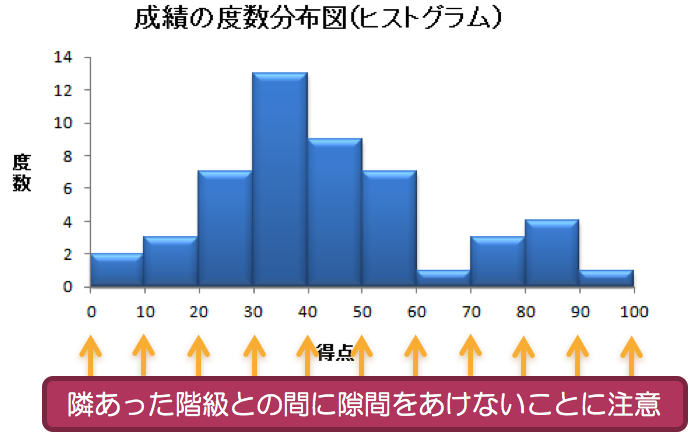
\includegraphics[width=0.5\textwidth,height=\textheight]{images/lec02/pic_hist_scores.png}
\caption{image of histogram}
\end{figure}

\begin{quote}
定義:スタージス(Sturges)の公式による階級の幅の決め方

\begin{enumerate}
\def\labelenumi{\arabic{enumi}.}
\tightlist
\item
  階級の数\(m\)を決定する:データ数が\(n\)のとき,適切な階級数\(m\)は
  \[
  m \approx 1+\frac{\log_{10} n}{\log_{10} 2} \approx 1+3.32 \log_{10} n
  \]
  なお,\(\approx\)は\textbf{ほぼ等しい}の意味。(参考:\(\log_{10} 2 \approx 0.301\))
\item
  階級の幅\(c\)を決定する:適切な級間隔\(c\)は
  \[
  c \approx \frac{x_{\max}-x_{\min}}{1+3.32 \log_{10} n}=\frac{\text{データの範囲}}{\text{階級数}}
  \]
\end{enumerate}
\end{quote}

\begin{itemize}
\tightlist
\item
  データの値の中で最も大きな値を\texttt{最大値(maximum)\textquotesingle{}\textquotesingle{},逆に最も小さな値を}最小値(minimum)'\,'とよびます
\item
  最大値と最小値の間隔を``データの範囲(range)'\,'とよびます
\end{itemize}

\begin{quote}
問題:学生の成績データ(スタージスの公式)
学生50人の成績データ(単位:点数)では最低点は5点,最高点は99点でした。スタージスの公式を使って,適切な階級数\(m\)と階級の幅\(c\)を求めて下さい
\end{quote}

\textbf{解答}

\begin{enumerate}
\def\labelenumi{\arabic{enumi}.}
\tightlist
\item
  スタージスの公式に必要な情報は次の通り
\end{enumerate}

\begin{longtable}[]{@{}lll@{}}
\toprule()
名称 & 記号 & 数値 \\
\midrule()
\endhead
データ数 & \(n\) & 50 \\
最大値 & \(x_{max}\) & 99 \\
最小値 & \(x_{min}\) & 5 \\
\bottomrule()
\end{longtable}

\begin{enumerate}
\def\labelenumi{\arabic{enumi}.}
\setcounter{enumi}{1}
\item
  適切な階級の数\(m\)は
  \[
  m 
  \approx 1+3.32 \times \log_{10} \mathop{50}_{\substack{\uparrow \\ n}}
  \approx 1+3.32 \times 1.699
  \approx 1+5.64 = 6.64
  \]
\item
  適切な級間隔\(c\)は
  \[
  c 
  \approx \frac{\text{データの範囲}}{\text{階級数}}
  \approx \frac{99-5}{7} 
  \approx 13
  \]
\end{enumerate}

\begin{quote}
階級の数の決め方の注意点
\end{quote}

\begin{enumerate}
\def\labelenumi{\arabic{enumi}.}
\tightlist
\item
  階級の「数」と「幅」は反比例の関係にある
\end{enumerate}

\begin{longtable}[]{@{}llll@{}}
\toprule()
階級の数 & 階級の幅 & ヒストグラム & 問題点 \\
\midrule()
\endhead
少なくする & 広くなる & 大雑把になる & 情報の喪失が大 \\
多くする & 狭くなる & 細かくなる & 情報を集約できない \\
\bottomrule()
\end{longtable}

\begin{enumerate}
\def\labelenumi{\arabic{enumi}.}
\setcounter{enumi}{1}
\item
  適切な階級の数と幅を決定するときにスタージスの公式を参考にするといい
\item
  次のような幅を設定することがポイント

  \begin{enumerate}
  \def\labelenumii{\arabic{enumii}.}
  \tightlist
  \item
    データ全体の傾向は損なわず、整理しやすい手頃な幅
  \item
    級間隔が直感的に分かりやすい幅
  \end{enumerate}
\end{enumerate}

\hypertarget{ux5ea6ux6570ux5206ux5e03ux8868ux304bux3089ux308fux304bux308bux3053ux3068}{%
\subsection{度数分布表からわかること}\label{ux5ea6ux6570ux5206ux5e03ux8868ux304bux3089ux308fux304bux308bux3053ux3068}}

\begin{quote}
問題:学生の成績データ(度数分布表の解釈)
先ほど作成した学生の成績データの\textbf{度数分布表}を参照しながら以下の値を求めて下さい

\begin{enumerate}
\def\labelenumi{\arabic{enumi}.}
\tightlist
\item
  点数が30点台の学生は何人いますか?
\item
  点数が30点台の学生は全体の何パーセントですか?
\item
  50点未満の学生は何人いますか?
\item
  50点未満の学生は何パーセントですか?
\end{enumerate}
\end{quote}

\textbf{解答}
1. 13人
2. 26パーセント
3. 34人
4. 68パーセント

\begin{quote}
問題:学生の成績データ(相対度数)
点数が31点から40点の学生は全体の何パーセントですか?
\end{quote}

\[
\text{30点台の階級の相対度数}
=\frac{\text{30点台の階級の度数}}{\text{全度数}}
=\frac{13}{50}=0.26
\]

\begin{quote}
定義:相対度数分布
\textbf{相対度数}の分布を表示したもの
\end{quote}

\begin{longtable}[]{@{}rrcl@{}}
\toprule()
階級(点) & 度数(人) & 相対度数 & \\
\midrule()
\endhead
0-9 & 2 & 0.04 & \(\leftarrow 2/50\) \\
10-19 & 3 & 0.06 & \(\leftarrow 3/50\) \\
20-29 & 7 & 0.14 & \\
30-39 & 13 & 0.26 & \(\leftarrow 13/50\) \\
40-49 & 9 & 0.18 & \\
50-59 & 7 & 0.14 & \\
60-69 & 1 & 0.02 & \\
70-79 & 3 & 0.06 & \\
80-89 & 4 & 0.08 & \\
90-99 & 1 & 0.02 & \\
合計 & 50 & 1.00 & \\
\bottomrule()
\end{longtable}

\hypertarget{ux30edux30fcux30ecux30f3ux30c4ux66f2ux7dda}{%
\chapter{ローレンツ曲線}\label{ux30edux30fcux30ecux30f3ux30c4ux66f2ux7dda}}

\begin{quote}
定義:(所得の)5分位階級
全ての世帯を所得の低い方から順番に並べ,それを世帯数で五等分して五つのグループを作った場合の各グループのことで,収入の低い方から順次第1,第2,第3,第4,第5分位階級とよぶ(参考:総務省,家計調査\textasciitilde 用語の解説 \url{http://www.stat.go.jp/data/kakei/kaisetsu.htm})
\end{quote}

\begin{quote}
問題:アメリカの1966年時点の所得の分布
次はアメリカの1966年時点の5分位階級別の所得の割合(\%)を示したデータです。コメントして下さい。
\end{quote}

\begin{longtable}[]{@{}llllll@{}}
\toprule()
所得階級 & 第1分位 & 第2分位 & 第3分位 & 第4分位 & 第5分位 \\
\midrule()
\endhead
1966年 & 5.6 & 12.4 & 17.7 & 23.8 & 40.5 \\
\bottomrule()
\end{longtable}

出所:US Department of Commerce, Statistical Abstract of the United States

\begin{quote}
定義:円グラフ(パイチャート)
360度の円を,100分比に応じて中心点から扇状に区切ったグラフ表現のこと。構成比を表すのに適したグラフ
\end{quote}

\begin{figure}
\centering
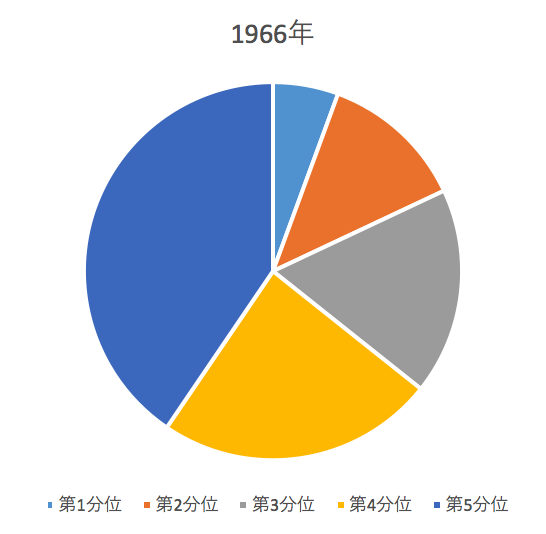
\includegraphics[width=0.5\textwidth,height=\textheight]{images/lec03/fig_us_income_dist1966.png}
\caption{image of histogram}
\end{figure}

\begin{quote}
問題:アメリカの1966年時点の所得の分布
世帯数と所得の累積比率を計算し,コメントして下さい
\end{quote}

\textbf{解答}

~~~~~~~~~\textbar{} 所得分配 \textbar{} 累積比率 \textbar{} 累積比率 \textbar{}\\
所得階級 \textbar{} 1966年 \textbar{} 世帯数 \textbar{} 所得 \textbar{}\\
--- \textbar{} --- \textbar{} --- \textbar{} --- \textbar{}\\
第1分位 \textbar{} 0.056 \textbar{} 0.200 \textbar{} 0.056 \textbar{}\\
第2分位 \textbar{} 0.124 \textbar{} 0.400 \textbar{} 0.180 \textbar{}\\
第3分位 \textbar{} 0.177 \textbar{} 0.600 \textbar{} 0.357 \textbar{}\\
第4分位 \textbar{} 0.238 \textbar{} 0.800 \textbar{} 0.595 \textbar{}\\
第5分位 \textbar{} 0.405 \textbar{} 1.000 \textbar{} 1.000 \textbar{}

\begin{itemize}
\tightlist
\item
  第1分位は所得全体の5.6\%
\item
  所得が低い方から6割の世帯(第3分位までの世帯)の所得は,全体の4割未満(35.7\%)
\item
  所得が多い上位20\%の世帯が,全所得の4割程度を獲得している
\end{itemize}

\begin{quote}
問題:アメリカの1966年時点の所得の分布
1966年時点のアメリカの所得分配は不平等のように思えます。では逆に,完全に平等な場合の,(1)円グラフ,(2)累積比率はどうなりますか
\end{quote}

\begin{figure}
\centering
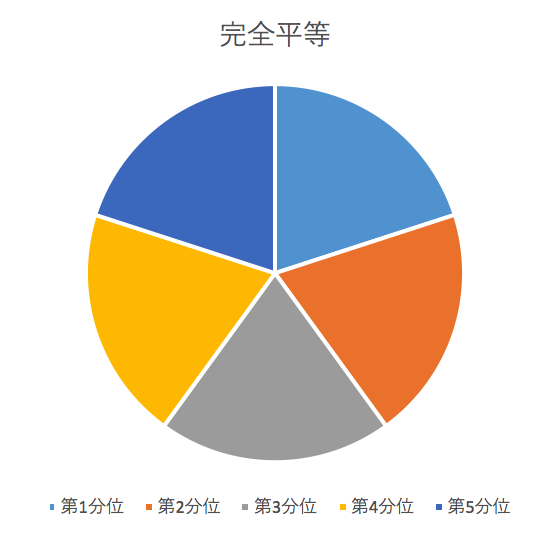
\includegraphics[width=0.5\textwidth,height=\textheight]{images/lec03/fig_income_dist_perfectly_equal.png}
\caption{image of histogram}
\end{figure}

\begin{quote}
問題:アメリカの1966年時点の所得の分布
所得分配の不平等度を的確に表す方法は?
\end{quote}

\begin{quote}
定義:ローレンツ曲線
ローレンツ曲線(Lorenz curve)は,所得分布や資産分布などの格差,不平等度,集中度を明らかにするための代表的な方法で,1905年にアメリカの統計学者ローレンツ(M.O.Lorenz)によって考案されました
\end{quote}

\begin{quote}
累積世帯比率と累積所得比率
\end{quote}

\hypertarget{ux30edux30fcux30ecux30f3ux30c4ux66f2ux7ddaux3068ux30b8ux30cbux4fc2ux6570}{%
\subsection{ローレンツ曲線とジニ係数}\label{ux30edux30fcux30ecux30f3ux30c4ux66f2ux7ddaux3068ux30b8ux30cbux4fc2ux6570}}

\begin{figure}
\centering
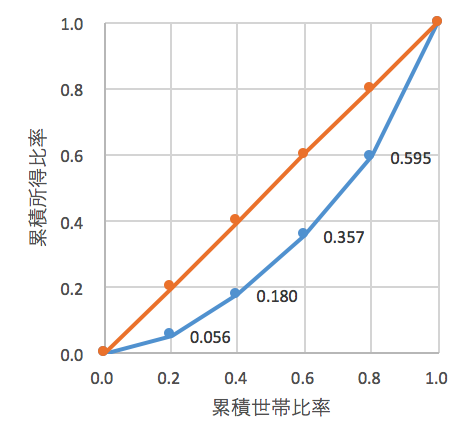
\includegraphics[width=0.5\textwidth,height=\textheight]{images/lec03/fig_us_lorenz1966.png}
\caption{image of histogram}
\end{figure}

\begin{quote}
ポイント

\begin{enumerate}
\def\labelenumi{\arabic{enumi}.}
\tightlist
\item
  青線が1966年のデータから計算した\textbf{ローレンツ曲線}です
\item
  オレンジ線を\textbf{完全平等線}とよびます
\item
  \textbf{所得分配が平等化}してくるとローレンツ曲線は完全平等線に\textbf{接近}します
\item
  オレンジと青の線の間の\textbf{領域が広いほど不平等度が高く}なります
\item
  2本の線に挟まれた\textbf{領域の面積の2倍の値をジニ係数}とよびます
\end{enumerate}
\end{quote}

\begin{quote}
確認問題:2005年のアメリカの所得分布
2005年の数値を使ってローレンツ曲線を描き,結果についてコメントして下さい
\end{quote}

所得階級 \& 第1分位 \& 第2分位 \& 第3分位 \& 第4分位 \& 第5分位 \textbackslash{}
2005年 \& 4.0 \& 9.6 \& 15.3 \& 23.0 \& 48.1 \textbackslash{}
出所:US Department of Commerce, Statistical Abstract of the United States

\textbf{解答}

\begin{figure}
\centering
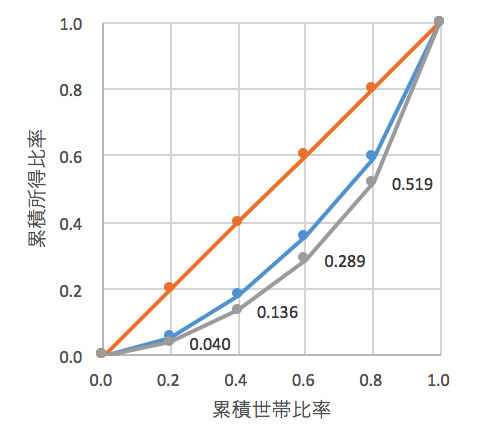
\includegraphics[width=0.5\textwidth,height=\textheight]{images/lec03/fig_us_lorenz2005.png}
\caption{image of histogram}
\end{figure}

\begin{itemize}
\tightlist
\item
  1969年から2005年にかけて,ローレンツ曲線は完全平等線からさらに離れている
\item
  このことから,1966年から2005年にかけて所得分布の不平等化が進んでいることがうかがわれる
\end{itemize}

\hypertarget{ux30b8ux30cbux4fc2ux6570}{%
\section{ジニ係数}\label{ux30b8ux30cbux4fc2ux6570}}

\begin{quote}
定義:ジニ係数

\begin{enumerate}
\def\labelenumi{\arabic{enumi}.}
\tightlist
\item
  ジニ係数(Gini coefficient)はローレンツ曲線のかたちを計測可能な指数にしたもので,(所得分配などの)分布の不平等度,集中度を示す指標です。
\item
  ジニ係数は\textbf{0から1のあいだの値}をとり,0に近いほど平等に近く,1に近いほど不平等度が大きいことを意味します
\end{enumerate}
\end{quote}

\begin{quote}
ジニ係数の計算方法

\begin{enumerate}
\def\labelenumi{\arabic{enumi}.}
\tightlist
\item
  完全平等線より右下の領域(領域A)の面積は0.5
\item
  ローレンツ曲線よりも右下の領域Bの面積を求める
\end{enumerate}
\end{quote}

\begin{align*}
\text{ジニ係数}
=(\text{領域Aの面積}-\text{領域Bの面積})\times 2
=1-\text{領域Bの面積}\times 2 
\end{align*}

\begin{quote}
\begin{enumerate}
\def\labelenumi{\arabic{enumi}.}
\setcounter{enumi}{2}
\tightlist
\item
  ローレンツ曲線よりも右下の領域の面積の計算方法
\end{enumerate}
\end{quote}

\begin{figure}
\centering
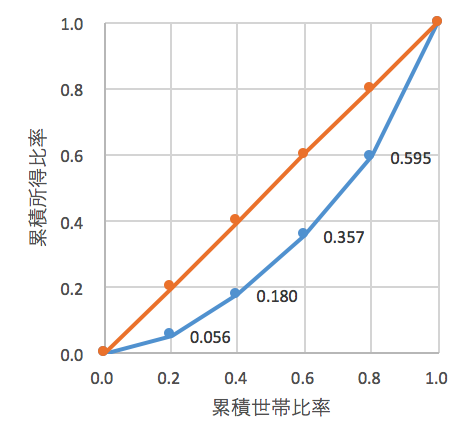
\includegraphics[width=0.5\textwidth,height=\textheight]{images/lec03/fig_us_lorenz1966.png}
\caption{image of histogram}
\end{figure}

\begin{itemize}
\tightlist
\item
  領域を5分割し,三角形と台形の面積を求め,合計します
\end{itemize}

\begin{align*} 
&\tfrac{1}{2} \times \mathop{0.056}_{\substack{\uparrow \\ \text{底辺}}} \times \mathop{0.2}_{\substack{\uparrow \\ \text{高さ}}} \\
&+\tfrac{1}{2} \times (0.056+0.180) \times 0.2 \\
&+\tfrac{1}{2} \times (0.180+0.357) \times 0.2 \\
&+\tfrac{1}{2} \times (0.357+0.595) \times 0.2 \\
&+\tfrac{1}{2} \times (
\mathop{0.595}_{\substack{\uparrow \\ \text{上底}}}
+
\mathop{1.000}_{\substack{\uparrow \\ \text{下底}}}
) \times 
\mathop{0.2}_{\substack{\uparrow \\ \text{高さ}}} \\
&=0.3376
\end{align*}

\begin{enumerate}
\def\labelenumi{\arabic{enumi}.}
\setcounter{enumi}{3}
\item
  よって1969年のジニ係数は
  \begin{align*}
  \text{ジニ係数}=1-0.3376\times 2=0.3248
  \end{align*}
\item
  領域Bの計算のコツ
\end{enumerate}

\begin{itemize}
\item
  今回の例では,5分位の世帯比率を使っているため,累積世帯比率は20\%ずつ等間隔で増加します。そのため面積を計算するときの``高さ'\,'はすべて0.2です
\item
  さらに,三角形と台形の公式では\(\tfrac{1}{2}\)が共通です
\item
  これらの共通項を括り出せば
  \begin{align*} 
  &\tfrac{1}{2} \times \mathop{0.2}_{\substack{\uparrow \\ \text{高さ}}} \times 
  \{ 0.056+ (0.056+0.180)+ (0.180+0.357) \\
  &\qquad\qquad+(0.357+0.595)+(0.595+1.000) \} \\
  &=0.3376
  \end{align*}
\end{itemize}

\begin{quote}
確認問題:2005年のアメリカの所得分布
2005年の数値を使ってジニ係数を計算して下さい
\end{quote}

\textbf{解答}

\begin{enumerate}
\def\labelenumi{\arabic{enumi}.}
\item
  領域Bの面積は
  \begin{align*}
  \text{領域Bの面積}
  &=\tfrac{1}{2} \times \mathop{0.2}_{\substack{\uparrow \\ \text{高さ}}} \times 
  \{ 0.040+ (0.040+0.136) \\
  &\qquad\qquad+(0.136+0.289)+(0.289+0.519) \\
  &\qquad\qquad+(0.519+1.000) \} \\
  &=0.2968
  \end{align*}
\item
  したがって2005年のジニ係数は
  \begin{align*}
  \text{ジニ係数}
  =1-2 \times 0.2968
  =0.4064
  \end{align*}
\item
  解釈:ジニ係数の値は0.3248(1969年)から0.4064(2005年)へ上昇しており,所得分配の不平等化がすすんだ
\end{enumerate}

\hypertarget{part-ux7b2cuxff12ux90e8}{%
\chapter{(PART*) 第2部}\label{part-ux7b2cuxff12ux90e8}}

\hypertarget{hello-bookdown}{%
\chapter{Hello bookdown}\label{hello-bookdown}}

All chapters start with a first-level heading followed by your chapter title, like the line above. There should be only one first-level heading (\texttt{\#}) per .Rmd file.

\hypertarget{a-section}{%
\section{A section}\label{a-section}}

All chapter sections start with a second-level (\texttt{\#\#}) or higher heading followed by your section title, like the sections above and below here. You can have as many as you want within a chapter.

\hypertarget{an-unnumbered-section}{%
\subsection*{An unnumbered section}\label{an-unnumbered-section}}
\addcontentsline{toc}{subsection}{An unnumbered section}

Chapters and sections are numbered by default. To un-number a heading, add a \texttt{\{.unnumbered\}} or the shorter \texttt{\{-\}} at the end of the heading, like in this section.

\hypertarget{hello-bookdown-1}{%
\chapter{Hello bookdown}\label{hello-bookdown-1}}

All chapters start with a first-level heading followed by your chapter title, like the line above. There should be only one first-level heading (\texttt{\#}) per .Rmd file.

\hypertarget{a-section-1}{%
\section{A section}\label{a-section-1}}

All chapter sections start with a second-level (\texttt{\#\#}) or higher heading followed by your section title, like the sections above and below here. You can have as many as you want within a chapter.

\hypertarget{an-unnumbered-section-1}{%
\subsection*{An unnumbered section}\label{an-unnumbered-section-1}}
\addcontentsline{toc}{subsection}{An unnumbered section}

Chapters and sections are numbered by default. To un-number a heading, add a \texttt{\{.unnumbered\}} or the shorter \texttt{\{-\}} at the end of the heading, like in this section.

\hypertarget{hello-bookdown-2}{%
\chapter{Hello bookdown}\label{hello-bookdown-2}}

All chapters start with a first-level heading followed by your chapter title, like the line above. There should be only one first-level heading (\texttt{\#}) per .Rmd file.

\hypertarget{a-section-2}{%
\section{A section}\label{a-section-2}}

All chapter sections start with a second-level (\texttt{\#\#}) or higher heading followed by your section title, like the sections above and below here. You can have as many as you want within a chapter.

\hypertarget{an-unnumbered-section-2}{%
\subsection*{An unnumbered section}\label{an-unnumbered-section-2}}
\addcontentsline{toc}{subsection}{An unnumbered section}

Chapters and sections are numbered by default. To un-number a heading, add a \texttt{\{.unnumbered\}} or the shorter \texttt{\{-\}} at the end of the heading, like in this section.

\hypertarget{hello-bookdown-3}{%
\chapter{Hello bookdown}\label{hello-bookdown-3}}

All chapters start with a first-level heading followed by your chapter title, like the line above. There should be only one first-level heading (\texttt{\#}) per .Rmd file.

\hypertarget{a-section-3}{%
\section{A section}\label{a-section-3}}

All chapter sections start with a second-level (\texttt{\#\#}) or higher heading followed by your section title, like the sections above and below here. You can have as many as you want within a chapter.

\hypertarget{an-unnumbered-section-3}{%
\subsection*{An unnumbered section}\label{an-unnumbered-section-3}}
\addcontentsline{toc}{subsection}{An unnumbered section}

Chapters and sections are numbered by default. To un-number a heading, add a \texttt{\{.unnumbered\}} or the shorter \texttt{\{-\}} at the end of the heading, like in this section.

\hypertarget{hello-bookdown-4}{%
\chapter{Hello bookdown}\label{hello-bookdown-4}}

All chapters start with a first-level heading followed by your chapter title, like the line above. There should be only one first-level heading (\texttt{\#}) per .Rmd file.

\hypertarget{a-section-4}{%
\section{A section}\label{a-section-4}}

All chapter sections start with a second-level (\texttt{\#\#}) or higher heading followed by your section title, like the sections above and below here. You can have as many as you want within a chapter.

\hypertarget{an-unnumbered-section-4}{%
\subsection*{An unnumbered section}\label{an-unnumbered-section-4}}
\addcontentsline{toc}{subsection}{An unnumbered section}

Chapters and sections are numbered by default. To un-number a heading, add a \texttt{\{.unnumbered\}} or the shorter \texttt{\{-\}} at the end of the heading, like in this section.

\hypertarget{hello-bookdown-5}{%
\chapter{Hello bookdown}\label{hello-bookdown-5}}

All chapters start with a first-level heading followed by your chapter title, like the line above. There should be only one first-level heading (\texttt{\#}) per .Rmd file.

\hypertarget{a-section-5}{%
\section{A section}\label{a-section-5}}

All chapter sections start with a second-level (\texttt{\#\#}) or higher heading followed by your section title, like the sections above and below here. You can have as many as you want within a chapter.

\hypertarget{an-unnumbered-section-5}{%
\subsection*{An unnumbered section}\label{an-unnumbered-section-5}}
\addcontentsline{toc}{subsection}{An unnumbered section}

Chapters and sections are numbered by default. To un-number a heading, add a \texttt{\{.unnumbered\}} or the shorter \texttt{\{-\}} at the end of the heading, like in this section.

\hypertarget{hello-bookdown-6}{%
\chapter{Hello bookdown}\label{hello-bookdown-6}}

All chapters start with a first-level heading followed by your chapter title, like the line above. There should be only one first-level heading (\texttt{\#}) per .Rmd file.

\hypertarget{a-section-6}{%
\section{A section}\label{a-section-6}}

All chapter sections start with a second-level (\texttt{\#\#}) or higher heading followed by your section title, like the sections above and below here. You can have as many as you want within a chapter.

\hypertarget{an-unnumbered-section-6}{%
\subsection*{An unnumbered section}\label{an-unnumbered-section-6}}
\addcontentsline{toc}{subsection}{An unnumbered section}

Chapters and sections are numbered by default. To un-number a heading, add a \texttt{\{.unnumbered\}} or the shorter \texttt{\{-\}} at the end of the heading, like in this section.

\hypertarget{hello-bookdown-7}{%
\chapter{Hello bookdown}\label{hello-bookdown-7}}

All chapters start with a first-level heading followed by your chapter title, like the line above. There should be only one first-level heading (\texttt{\#}) per .Rmd file.

\hypertarget{a-section-7}{%
\section{A section}\label{a-section-7}}

All chapter sections start with a second-level (\texttt{\#\#}) or higher heading followed by your section title, like the sections above and below here. You can have as many as you want within a chapter.

\hypertarget{an-unnumbered-section-7}{%
\subsection*{An unnumbered section}\label{an-unnumbered-section-7}}
\addcontentsline{toc}{subsection}{An unnumbered section}

Chapters and sections are numbered by default. To un-number a heading, add a \texttt{\{.unnumbered\}} or the shorter \texttt{\{-\}} at the end of the heading, like in this section.

\hypertarget{hello-bookdown-8}{%
\chapter{Hello bookdown}\label{hello-bookdown-8}}

All chapters start with a first-level heading followed by your chapter title, like the line above. There should be only one first-level heading (\texttt{\#}) per .Rmd file.

\hypertarget{a-section-8}{%
\section{A section}\label{a-section-8}}

All chapter sections start with a second-level (\texttt{\#\#}) or higher heading followed by your section title, like the sections above and below here. You can have as many as you want within a chapter.

\hypertarget{an-unnumbered-section-8}{%
\subsection*{An unnumbered section}\label{an-unnumbered-section-8}}
\addcontentsline{toc}{subsection}{An unnumbered section}

Chapters and sections are numbered by default. To un-number a heading, add a \texttt{\{.unnumbered\}} or the shorter \texttt{\{-\}} at the end of the heading, like in this section.

\hypertarget{hello-bookdown-9}{%
\chapter{Hello bookdown}\label{hello-bookdown-9}}

All chapters start with a first-level heading followed by your chapter title, like the line above. There should be only one first-level heading (\texttt{\#}) per .Rmd file.

\hypertarget{a-section-9}{%
\section{A section}\label{a-section-9}}

All chapter sections start with a second-level (\texttt{\#\#}) or higher heading followed by your section title, like the sections above and below here. You can have as many as you want within a chapter.

\hypertarget{an-unnumbered-section-9}{%
\subsection*{An unnumbered section}\label{an-unnumbered-section-9}}
\addcontentsline{toc}{subsection}{An unnumbered section}

Chapters and sections are numbered by default. To un-number a heading, add a \texttt{\{.unnumbered\}} or the shorter \texttt{\{-\}} at the end of the heading, like in this section.

\hypertarget{hello-bookdown-10}{%
\chapter{Hello bookdown}\label{hello-bookdown-10}}

All chapters start with a first-level heading followed by your chapter title, like the line above. There should be only one first-level heading (\texttt{\#}) per .Rmd file.

\hypertarget{a-section-10}{%
\section{A section}\label{a-section-10}}

All chapter sections start with a second-level (\texttt{\#\#}) or higher heading followed by your section title, like the sections above and below here. You can have as many as you want within a chapter.

\hypertarget{an-unnumbered-section-10}{%
\subsection*{An unnumbered section}\label{an-unnumbered-section-10}}
\addcontentsline{toc}{subsection}{An unnumbered section}

Chapters and sections are numbered by default. To un-number a heading, add a \texttt{\{.unnumbered\}} or the shorter \texttt{\{-\}} at the end of the heading, like in this section.

\hypertarget{hello-bookdown-11}{%
\chapter{Hello bookdown}\label{hello-bookdown-11}}

All chapters start with a first-level heading followed by your chapter title, like the line above. There should be only one first-level heading (\texttt{\#}) per .Rmd file.

\hypertarget{a-section-11}{%
\section{A section}\label{a-section-11}}

All chapter sections start with a second-level (\texttt{\#\#}) or higher heading followed by your section title, like the sections above and below here. You can have as many as you want within a chapter.

\hypertarget{an-unnumbered-section-11}{%
\subsection*{An unnumbered section}\label{an-unnumbered-section-11}}
\addcontentsline{toc}{subsection}{An unnumbered section}

Chapters and sections are numbered by default. To un-number a heading, add a \texttt{\{.unnumbered\}} or the shorter \texttt{\{-\}} at the end of the heading, like in this section.

\hypertarget{hello-bookdown-12}{%
\chapter{Hello bookdown}\label{hello-bookdown-12}}

All chapters start with a first-level heading followed by your chapter title, like the line above. There should be only one first-level heading (\texttt{\#}) per .Rmd file.

\hypertarget{a-section-12}{%
\section{A section}\label{a-section-12}}

All chapter sections start with a second-level (\texttt{\#\#}) or higher heading followed by your section title, like the sections above and below here. You can have as many as you want within a chapter.

\hypertarget{an-unnumbered-section-12}{%
\subsection*{An unnumbered section}\label{an-unnumbered-section-12}}
\addcontentsline{toc}{subsection}{An unnumbered section}

Chapters and sections are numbered by default. To un-number a heading, add a \texttt{\{.unnumbered\}} or the shorter \texttt{\{-\}} at the end of the heading, like in this section.

\hypertarget{hello-bookdown-13}{%
\chapter{Hello bookdown}\label{hello-bookdown-13}}

All chapters start with a first-level heading followed by your chapter title, like the line above. There should be only one first-level heading (\texttt{\#}) per .Rmd file.

\hypertarget{a-section-13}{%
\section{A section}\label{a-section-13}}

All chapter sections start with a second-level (\texttt{\#\#}) or higher heading followed by your section title, like the sections above and below here. You can have as many as you want within a chapter.

\hypertarget{an-unnumbered-section-13}{%
\subsection*{An unnumbered section}\label{an-unnumbered-section-13}}
\addcontentsline{toc}{subsection}{An unnumbered section}

Chapters and sections are numbered by default. To un-number a heading, add a \texttt{\{.unnumbered\}} or the shorter \texttt{\{-\}} at the end of the heading, like in this section.

\hypertarget{cross}{%
\chapter{Cross-references}\label{cross}}

Cross-references make it easier for your readers to find and link to elements in your book.

\hypertarget{chapters-and-sub-chapters}{%
\section{Chapters and sub-chapters}\label{chapters-and-sub-chapters}}

There are two steps to cross-reference any heading:

\begin{enumerate}
\def\labelenumi{\arabic{enumi}.}
\tightlist
\item
  Label the heading: \texttt{\#\ Hello\ world\ \{\#nice-label\}}.

  \begin{itemize}
  \tightlist
  \item
    Leave the label off if you like the automated heading generated based on your heading title: for example, \texttt{\#\ Hello\ world} = \texttt{\#\ Hello\ world\ \{\#hello-world\}}.
  \item
    To label an un-numbered heading, use: \texttt{\#\ Hello\ world\ \{-\#nice-label\}} or \texttt{\{\#\ Hello\ world\ .unnumbered\}}.
  \end{itemize}
\item
  Next, reference the labeled heading anywhere in the text using \texttt{\textbackslash{}@ref(nice-label)}; for example, please see Chapter \ref{cross}.

  \begin{itemize}
  \tightlist
  \item
    If you prefer text as the link instead of a numbered reference use: \protect\hyperlink{cross}{any text you want can go here}.
  \end{itemize}
\end{enumerate}

\hypertarget{captioned-figures-and-tables}{%
\section{Captioned figures and tables}\label{captioned-figures-and-tables}}

Figures and tables \emph{with captions} can also be cross-referenced from elsewhere in your book using \texttt{\textbackslash{}@ref(fig:chunk-label)} and \texttt{\textbackslash{}@ref(tab:chunk-label)}, respectively.

See Figure \ref{fig:nice-fig}.

\begin{Shaded}
\begin{Highlighting}[]
\FunctionTok{par}\NormalTok{(}\AttributeTok{mar =} \FunctionTok{c}\NormalTok{(}\DecValTok{4}\NormalTok{, }\DecValTok{4}\NormalTok{, .}\DecValTok{1}\NormalTok{, .}\DecValTok{1}\NormalTok{))}
\FunctionTok{plot}\NormalTok{(pressure, }\AttributeTok{type =} \StringTok{\textquotesingle{}b\textquotesingle{}}\NormalTok{, }\AttributeTok{pch =} \DecValTok{19}\NormalTok{)}
\end{Highlighting}
\end{Shaded}

\begin{figure}

{\centering 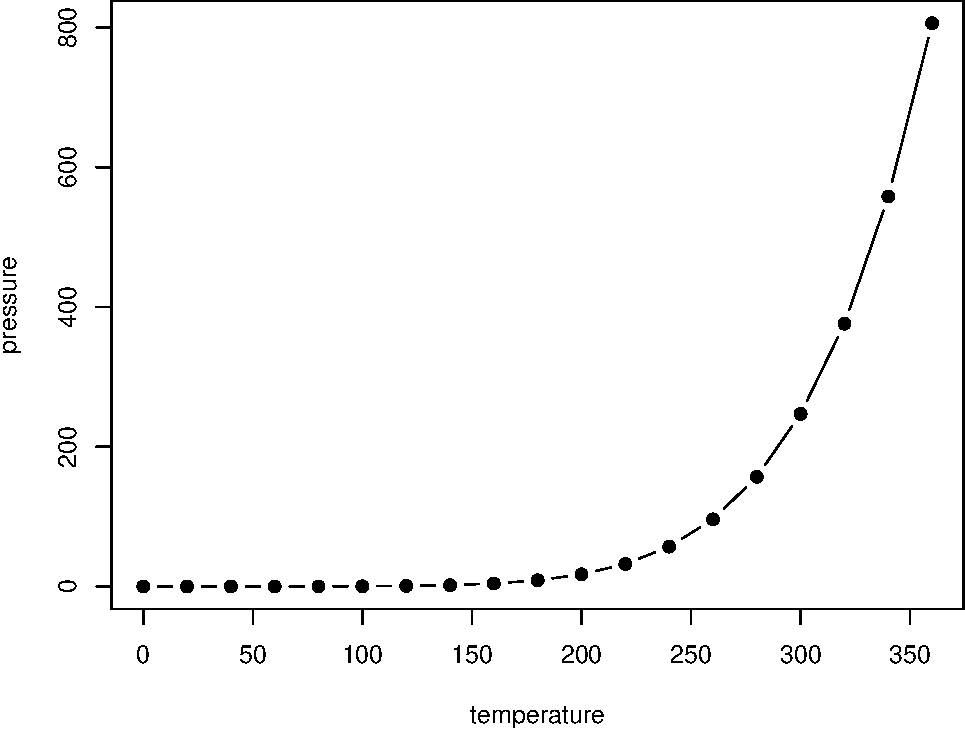
\includegraphics[width=0.8\linewidth]{t02-cross-refs_files/figure-latex/nice-fig-1} 

}

\caption{Here is a nice figure!}\label{fig:nice-fig}
\end{figure}

Don't miss Table \ref{tab:nice-tab}.

\begin{Shaded}
\begin{Highlighting}[]
\NormalTok{knitr}\SpecialCharTok{::}\FunctionTok{kable}\NormalTok{(}
  \FunctionTok{head}\NormalTok{(pressure, }\DecValTok{10}\NormalTok{), }\AttributeTok{caption =} \StringTok{\textquotesingle{}Here is a nice table!\textquotesingle{}}\NormalTok{,}
  \AttributeTok{booktabs =} \ConstantTok{TRUE}
\NormalTok{)}
\end{Highlighting}
\end{Shaded}

\begin{table}

\caption{\label{tab:nice-tab}Here is a nice table!}
\centering
\begin{tabular}[t]{rr}
\toprule
temperature & pressure\\
\midrule
0 & 0.0002\\
20 & 0.0012\\
40 & 0.0060\\
60 & 0.0300\\
80 & 0.0900\\
\addlinespace
100 & 0.2700\\
120 & 0.7500\\
140 & 1.8500\\
160 & 4.2000\\
180 & 8.8000\\
\bottomrule
\end{tabular}
\end{table}

\hypertarget{parts}{%
\chapter{Parts}\label{parts}}

You can add parts to organize one or more book chapters together. Parts can be inserted at the top of an .Rmd file, before the first-level chapter heading in that same file.

Add a numbered part: \texttt{\#\ (PART)\ Act\ one\ \{-\}} (followed by \texttt{\#\ A\ chapter})

Add an unnumbered part: \texttt{\#\ (PART\textbackslash{}*)\ Act\ one\ \{-\}} (followed by \texttt{\#\ A\ chapter})

Add an appendix as a special kind of un-numbered part: \texttt{\#\ (APPENDIX)\ Other\ stuff\ \{-\}} (followed by \texttt{\#\ A\ chapter}). Chapters in an appendix are prepended with letters instead of numbers.

\hypertarget{footnotes-and-citations}{%
\chapter{Footnotes and citations}\label{footnotes-and-citations}}

\hypertarget{footnotes}{%
\section{Footnotes}\label{footnotes}}

Footnotes are put inside the square brackets after a caret \texttt{\^{}{[}{]}}. Like this one \footnote{This is a footnote.}.

\hypertarget{citations}{%
\section{Citations}\label{citations}}

Reference items in your bibliography file(s) using \texttt{@key}.

For example, we are using the \textbf{bookdown} package \citep{R-bookdown} (check out the last code chunk in index.Rmd to see how this citation key was added) in this sample book, which was built on top of R Markdown and \textbf{knitr} \citep{xie2015} (this citation was added manually in an external file book.bib).
Note that the \texttt{.bib} files need to be listed in the index.Rmd with the YAML \texttt{bibliography} key.

The \texttt{bs4\_book} theme makes footnotes appear inline when you click on them. In this example book, we added \texttt{csl:\ chicago-fullnote-bibliography.csl} to the \texttt{index.Rmd} YAML, and include the \texttt{.csl} file. To download a new style, we recommend: \url{https://www.zotero.org/styles/}

The RStudio Visual Markdown Editor can also make it easier to insert citations: \url{https://rstudio.github.io/visual-markdown-editing/\#/citations}

\hypertarget{blocks}{%
\chapter{Blocks}\label{blocks}}

\hypertarget{equations}{%
\section{Equations}\label{equations}}

Here is an equation.

\begin{equation} 
  f\left(k\right) = \binom{n}{k} p^k\left(1-p\right)^{n-k}
  \label{eq:binom}
\end{equation}

You may refer to using \texttt{\textbackslash{}@ref(eq:binom)}, like see Equation \eqref{eq:binom}.

\hypertarget{theorems-and-proofs}{%
\section{Theorems and proofs}\label{theorems-and-proofs}}

Labeled theorems can be referenced in text using \texttt{\textbackslash{}@ref(thm:tri)}, for example, check out this smart theorem \ref{thm:tri}.

\begin{theorem}
\protect\hypertarget{thm:tri}{}\label{thm:tri}For a right triangle, if \(c\) denotes the \emph{length} of the hypotenuse
and \(a\) and \(b\) denote the lengths of the \textbf{other} two sides, we have
\[a^2 + b^2 = c^2\]
\end{theorem}

Read more here \url{https://bookdown.org/yihui/bookdown/markdown-extensions-by-bookdown.html}.

\hypertarget{callout-blocks}{%
\section{Callout blocks}\label{callout-blocks}}

The \texttt{bs4\_book} theme also includes special callout blocks, like this \texttt{.rmdnote}.

You can use \textbf{markdown} inside a block.

\begin{Shaded}
\begin{Highlighting}[]
\FunctionTok{head}\NormalTok{(beaver1, }\AttributeTok{n =} \DecValTok{5}\NormalTok{)}
\CommentTok{\#\textgreater{}   day time  temp activ}
\CommentTok{\#\textgreater{} 1 346  840 36.33     0}
\CommentTok{\#\textgreater{} 2 346  850 36.34     0}
\CommentTok{\#\textgreater{} 3 346  900 36.35     0}
\CommentTok{\#\textgreater{} 4 346  910 36.42     0}
\CommentTok{\#\textgreater{} 5 346  920 36.55     0}
\end{Highlighting}
\end{Shaded}

It is up to the user to define the appearance of these blocks for LaTeX output.

You may also use: \texttt{.rmdcaution}, \texttt{.rmdimportant}, \texttt{.rmdtip}, or \texttt{.rmdwarning} as the block name.

The R Markdown Cookbook provides more help on how to use custom blocks to design your own callouts: \url{https://bookdown.org/yihui/rmarkdown-cookbook/custom-blocks.html}

\hypertarget{sharing-your-book}{%
\chapter{Sharing your book}\label{sharing-your-book}}

\hypertarget{publishing}{%
\section{Publishing}\label{publishing}}

HTML books can be published online, see: \url{https://bookdown.org/yihui/bookdown/publishing.html}

\hypertarget{pages}{%
\section{404 pages}\label{pages}}

By default, users will be directed to a 404 page if they try to access a webpage that cannot be found. If you'd like to customize your 404 page instead of using the default, you may add either a \texttt{\_404.Rmd} or \texttt{\_404.md} file to your project root and use code and/or Markdown syntax.

\hypertarget{metadata-for-sharing}{%
\section{Metadata for sharing}\label{metadata-for-sharing}}

Bookdown HTML books will provide HTML metadata for social sharing on platforms like Twitter, Facebook, and LinkedIn, using information you provide in the \texttt{index.Rmd} YAML. To setup, set the \texttt{url} for your book and the path to your \texttt{cover-image} file. Your book's \texttt{title} and \texttt{description} are also used.

This \texttt{bs4\_book} provides enhanced metadata for social sharing, so that each chapter shared will have a unique description, auto-generated based on the content.

Specify your book's source repository on GitHub as the \texttt{repo} in the \texttt{\_output.yml} file, which allows users to view each chapter's source file or suggest an edit. Read more about the features of this output format here:

\url{https://pkgs.rstudio.com/bookdown/reference/bs4_book.html}

Or use:

\begin{Shaded}
\begin{Highlighting}[]
\NormalTok{?bookdown}\SpecialCharTok{::}\NormalTok{bs4\_book}
\end{Highlighting}
\end{Shaded}


  \bibliography{book.bib,packages.bib}

\end{document}
